% chapter2.tex
% Capitulo 2. Fundamentos teoricos
%==========================================================================
\chapter{Fundamentos te\'oricos}


%==========================================================================
\section{Concepto de se\~nal}

Una se\~nal se puede definir como una cantidad que se puede medir a trav\'es del
tiempo. Esta cantidad puede representar diversas cosas dependiendo de la
aplicaci\'on. Las se\~nales pueden ser de dos tipos: an\'alogas \'o discretas.
Las se\~nales an\'alogas, o tambi\'en conocidas como continuas, se pueden
definir como una funci\'on de valores reales o complejos, las cuales est\'an
definidas dentro de un intervalo de tiempo $t$. Este intervalo es normalmente 
infinito aunque tambi\'en se puede acotar a un
intervalo espec\'ifico, dependiendo del instante de tiempo que se desea medir. 
Las se\~nales discretas se definen como una funci\'on derivada de un conjunto de 
n\'umeros acotados a un intervalo espec\'ifico. Estos n\'umeros son las muestras
que se tomaron de la se\~nal en tiempos discretos. Esta informaci\'on es
almacenada como dato digital para posteriormente ser analizado y / o manipulado.
Un ejemplo de una se\~nal continua y discreta se muestra en la figura
\ref{fig:sine}.

\begin{figure}[ht]
\centering
	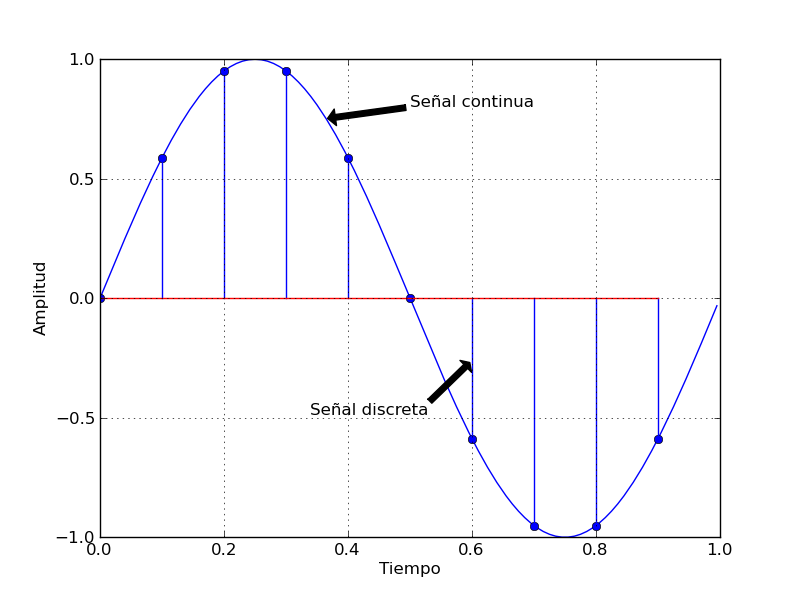
\includegraphics[width=5in]{figs/sine}
	\caption{Ejemplo de una se\~nal continua y una se\~nal discreta}
	\label{fig:sine}
\end{figure}

Una se\~nal puede ser determin\'istica o aleatoria. Se le denomina
determin\'istica a una se\~nal la cual no existe ninguna incertidumbre con
respecto a su valor dentro de un lapso de tiempo. Las se\~nales
determin\'isticas pueden ser expresadas por ecuaciones matem\'aticas, tales como
$x(t)=5\cos(10t)$. No es posible utilizar este tipo de ecuaciones para describir
se\~nales aleatorias, tambi\'en conocidas como procesos aleatorios, aunque s\'i 
es posible analizarlas utilizando m\'etodos estad\'isticos y de probabilidad
\cite{sklar}.

Las se\~nales tambi\'en pueden ser peri\'odicas o no peri\'odicas. Se dice que
una se\~nal es peri\'odica si existe una constante $T_0 > 0$ tal que la
siguiente ecuaci\'on se pueda satisfacer:
\begin{equation}\label{e:periodic}
x(t)=x(t+T_0) \quad   -\infty<t<\infty
\end{equation}

donde $t$ es el tiempo. El valor m\'as peque\~no de $T_0$ que pueda satisfacer
la ecuaci\'on \eqref{e:periodic} se le conoce como el periodo de $x(t)$. Una
se\~nal a la cual no existe un valor $T_0$ que satisfaga la ecuaci\'on
\eqref{e:periodic} se le denomina no peri\'odica \cite{sklar}.

Algunos ejemplos de varios tipos de se\~nales se muestran en la tabla
\ref{tbl:signals}.

\begin{table}[ht]
\begin{center}
	\begin{tabular}{|p{6cm}|p{7.3cm}|}
		\hline
		Variaciones en tiempo y espacio en una dimensi\'on (1D) &
		\begin{itemize}
		  \item Ac\'usticos: Se\~nales sonoras, eco de murci\'elagos y delfines.
		  \item Ingenier\'ia Electr\'onica: Se\~nales emitidas por una antena de
		  transmisi\'on.
		  \item Qu\'imica: Temperatura de una reacci\'on qu\'imica.
		  \item Finanzas: Historial del mercado de acciones.
		  \item Medicina: Se\~nales de un electrocardiograma.
		\end{itemize} \\
		\hline
		Variaciones en el espacio de dos dimensiones (2D) &
		\begin{itemize}
		  \item Ingenier\'ia de Agricultura: vegetaci\'on y evaporaci\'on en un campo.
		  \item Geograf\'ia: temperatura de la superficie y mapas de presi\'on.
		  \item Ingenier\'ia de Tr\'afico: taza de accidentes en un d\'ia de una
		  ciudad.
		\end{itemize} \\
		\hline
		Variaciones volum\'etricas de tres dimensiones (3D) &
		\begin{itemize}
		  \item Mec\'anica de fluidos: perfil de flujo-velocidad de un ala de un
		  avi\'on.
		  \item Biolog\'ia: distribuci\'on CO\textsubscript{2} de un bioreactor.
		\end{itemize} \\
		\hline
	\end{tabular}
	\vspace{0.5in}
	\caption{Ejemplos de se\~nales}
	\label{tbl:signals}
\end{center}
\end{table}

% 2.2 Sistema de comunicaciones digitales
%==========================================================================
\newpage
\section{Sistema de comunicaciones digitales}

Los componentes t\'ipicos de un sistema de comunicaciones digitales se muestran
en la figura \ref{fig:siscom}.

\begin{figure}[hpt]
\centering
	\begin{tikzpicture}[scale=0.8, transform shape, node distance = 20mm and 10mm, pin distance=10mm,
	inpin/.style={pin={[pin distance=10mm,pin edge={<-,black, very thick}]left:Mensaje a enviar}},
	outpin/.style={pin={[pin distance=10mm,pin edge={->,black, very thick}]left:Mensaje recibido}}]
		\node (format) [sc, inpin] {Formato de mensaje};
		\node (mod) [sc, right=of format] {Modulaci\'on por pulsos}
			edge[<-, very thick] (format);
		\node (modpass) [sc, right=of mod] {Modulaci\'on pasa bandas}
			edge[<-, very thick] (mod);
		\node[coordinate] (out) [right=of modpass]{};
		\draw[very thick] (modpass) -- (out) \antenna;
		
		\node (formatin) [sc, outpin, below=of format] {Formato de mensaje};
		\node (detect) [sc, right=of formatin] {Detecci\'on}
			edge [->, very thick] (formatin);
		\node (demod) [sc, right=of detect] {Demodulaci\'on y muestreo}
			edge [->, very thick] (detect);
		\draw[very thick] (demod.east) -- ++(1,0) \antenna;
	\end{tikzpicture}
	\vspace{0.3in}
	\caption{Diagrama a bloques de un sistema de comunicacion digital con transmisi\'on de datos pasa banda}
	\label{fig:siscom}
\end{figure}

La informaci\'on que se desea enviar es convertida en d\'igitos binarios en la
etapa de Formato de Mensaje. Estos d\'igitos son agrupados para formar mensajes
digitales o s\'imbolos para poder asegurar compatibilidad entre la informaci\'on
y el procesamiento de se\~nales dentro del sistema de comunicaciones digitales.
Hasta este punto la informaci\'on permanece en forma de una cadena de bits. La
modulaci\'on transforma los s\'imbolos del mensaje en formas de onda compatibles
con el canal de transmisi\'on. El bloque modulaci\'on por pulsos es importante
porque los s\'imbolos deben ser convertidos de una representaci\'on binaria a
una se\~nal banda base. Este t\'ermino se refiere a una se\~nal cuyo espectro
va desde 0 (o casi 0 o dc) hasta un valor finito, normalmente menos de unos
cuantos megahertz. Para una aplicaci\'on que involucre la transmisi\'on por RF, el
siguiente bloque es requerido cuando el canal no soporta la propagaci\'on de
se\~nales en forma de pulsos. Para tales casos se requiere la presencia de
se\~nales pasa bandas. Este t\'ermino se refiere a una se\~nal banda base cuya
frecuencia es traducida por una se\~nal portadora a una frecuencia mucho mayor
que su frecuencia original. La se\~nal recibida puede ser interpretada como
\begin{equation}\label{eq:mod}
r(t)=s_i(t)*h_c(t)+n(t) \qquad i=1,\ldots,M
\end{equation}
donde el operador $*$ representa una operaci\'on de convoluci\'on, $h_c(t)$
representa la respuesta al impulso del canal, $s_i(t)$ es la se\~nal transmitida
y $n(t)$ representa un proceso de ruido.

En el lado del receptor, el demodulador restablece $r(t)$ en pulsos banda base
\'optimamente formados $z(t)$ en preparaci\'on para ser detectados. Algunos
autores utilizan el t\'ermino demodulaci\'on y detecci\'on intercambiable y
otros definen la demodulaci\'on como el proceso de recuperaci\'on de la forma de
onda (pulso banda base), y detecci\'on como el proceso de toma de decisi\'on
sobre el significado digital de la forma de onda.

% 2.3 Concepto de modulador
%==========================================================================
\section{Concepto de modulador}

En el campo de las telecomunicaciones, la modulaci\'on es el proceso de variar
una forma de onda peri\'odica para enviar alg\'un tipo de mensaje. La necesidad
de modular una secuencia de datos para ser transmitida es relativa tama\~no de
la antena. Es posible transmitir una se\~nal sin antes haber sido modulada, pero
el tama\~no de la antena para poderla transmitir ser\'ia muy grande que no
ser\'ia factible la transmisi\'on. Por ejemplo, las se\~nales de tel\'efonos
celulares. El tama\~no de las antenas son t\'ipicamente $1/4$ de la longitud de onda
\cite{sklar}. Si consideramos una se\~nal de 3000Hz acopl\'andola directamente
sin haberla modulado antes, el tama\~no de la antena se puede calcular
utilizando la siguiente expresi\'on:
\begin{equation}
\begin{aligned}
\lambda=\frac{c}{f}&=\frac{3\times10^8m/s}{3000Hz}\\
\frac{\lambda}{4}&=2.5\times10^4m
\end{aligned}
\end{equation}
Si la se\~nal se modula antes de enviarla con una portadora o envolvente de
mayor frecuencia a la se\~nal que se desea enviar, por ejemplo 900Mhz, el
di\'ametro de la antena ser\'a de 8cm. Por esta raz\'on la modulaci\'on es un
paso esencial en todos los sistemas que involucran transmisi\'on de datos por
radio.

Otro beneficio que ofrece la modulaci\'on es de poder colocar la frecuencia de la se\~nal en otra
donde los requerimientos de filtrado y amplificaci\'on, entre otros requerimientos de dise\~no,
puedan ser logrados de una manera mas eficiente. Este es el caso donde por ejemplo, en el receptor,
la se\~nal de RF que es recibida es convertida a una frecuencia intermedia (IF) para que el sistema
pueda procesarla correctamente.

% 2.4 Envolvente compleja
%==========================================================================
\section{Envolvente compleja}

La descripci\'on de moduladores y demoduladores en la vida real se ha facilitado
por el uso de la notaci\'on compleja. Cualquier forma de onda pasa banda $s(t)$ 
puede ser representada utilizando la notaci\'on compleja \cite{sklar}
\begin{equation}\label{eq:complex}
s(t)=Re\{g(t)e^{j\theta(t)}\}
\end{equation}
donde $g(t)$ se conoce como la envolvente compleja, expresada como
\begin{equation}\label{eq:comcar}
g(t)=x(t)+jy(t)=\|g(t)\|e^{j\theta(t)}=R(t)e^{j\theta(t)}
\end{equation}
la magnitud de la envolvente es
\begin{equation}\label{eq:mag}
R(t)=\|g(t)\|=\sqrt{x^2(t)+y^2(t)}
\end{equation}
y su fase es
\begin{equation}\label{eq:fase}
\theta(t)=\tan^{-1}\frac{y(t)}{x(t)}
\end{equation}
Observando la ecuaci\'on \eqref{eq:complex} se dice que $g(t)$ es el mensaje de
la informaci\'on que se desea transmitir en forma compleja y $e^{j\theta t}$ es la
envolvente en su forma compleja. El producto de estas dos representa la
modulaci\'on y $s(t)$, la parte real del producto, es la forma de onda
transmitida. Con esto podemos expresar $s(t)$ de la siguiente manera
\cite{sklar}
\begin{equation}\label{eq:compsimple}
\begin{aligned}
s(t)&=Re\{(x(t)+jy(t))(\cos\omega_0t+j\sin\omega_0t)\}\\
s(t)&=x(t)\cos\omega_0t-y(t)\sin\omega_0t
\end{aligned}
\end{equation}

%==========================================================================
\section{El ruido como factor de degradaci\'on de la se\~nal transmitida}

El proceso de demodulaci\'on consiste en recuperar la informaci\'on (bits) de la se\~nal
transmitida con la menor cantidad de errores posible. Estos errores son causados por el ruido, el
cual se puede definir como cualquier distorsi\'on no deseada en la se\~nal. Podemos considerar dos
causas principales de ruido. La primera es debido al filtrado que se emplea en el transmisor, canal
y receptor. Si la funci\'on de transferencia de estos filtros no es la ideal pueden llegar a causar
un fen\'omeno conocido como interferencia entre s\'imbolos (ISI). La otra causa de degradaci\'on de
la se\~nal es debido a la interferencia generada por el medio ambiente incluyendo interferencia con
otras se\~nales. Existe un fen\'omeno natural que no se puede eliminar ni controlar denominado
\emph{ruido t\'ermico}. Este tipo de ruido es generado por el movimiento t\'ermico de los electrones
en cualquier medio conductor y puede ser descrito como un proceso aleatorio Gausseano con media cero, o sea, $\mu=0$. Un
proceso Gausseano $n(t)$ es una funci\'on aleatoria el cual su valor $n$ en cualquier punto en un tiempo $t$ esta
caracterizado por la funci\'on de densidad de probabilidad (PDF)

\begin{equation}\label{eq:gauss}
p(n)=\frac{1}{\sigma\sqrt{2\pi}}\exp\left[-\frac{1}{2}\left(\frac{n}{\sigma}\right)^2\right]
\end{equation}

donde $\sigma^2$ es la varianza de la muestra $n$. Su representaci\'on gr\'afica se muestra en la figura \ref{fig:gauss}.

\begin{figure}[ht]
\centering
	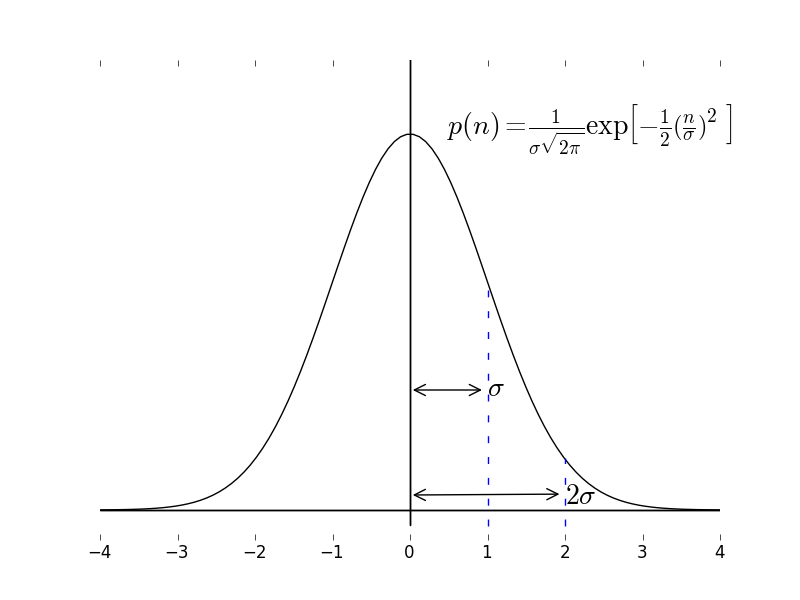
\includegraphics[width=5.5in]{figs/gauss}
	\caption{Funci\'on de densidad de probabilidad de la distribuci\'on Gaussiana}
	\label{fig:gauss}
\end{figure}

Otra caracter\'istica del ruido t\'ermico es que su distribuci\'on de potencia es igual para
todas las frecuencias, en otras palabras, su potencia esta uniformemente distribuida a trav\'es de
todo el espectro. Esta caracter\'istica le da el nombre ruido blanco.

Este ruido est\'a presente en todos los sistemas de comunicaci\'on y recibe el nombre de AWGN, as\'i
agrupando todas las caracter\'isticas anteriormente mencionadas (A de aditivo, W \emph{white} o
blanco y G de Gaussiano).

Si consideramos un sistema de comunicaciones binario que envia un 1 o un 0 en un intervalo de
s\'imbolo $T$

\begin{equation}\label{eq:binarycom}
s_i(t)=\left\{
\begin{array}{l l l}
s_1(t) & \quad 0\leq t \leq T & \quad \mbox{binario 1}\\
s_2(t) & \quad 0\leq t \leq T & \quad \mbox{binario 0}\\
\end{array}\right.
\end{equation}

y le agregamos ruido aditivo blanco la se\~nal recibida ser\'a

\begin{equation}\label{eq:signoise}
r(t)=s_i(t)+n(t) \quad i=1,2 \quad 0\leq t \leq T
\end{equation}

donde $s_i(t)$ es el s\'imbolo recibido y $n(t)$ es el ruido aleatorio causado por el movimiento de
los electrones.

Las caracter\'isticas del ruido AWGN son comunmente utilizadas para modelar la interferencia en
el proceso de detecci\'on y tambien para el dise\~no de receptores, ya que este tipo de ruido
siempre est\'a presente en todos los sistemas de comunicaciones y, por lo tanto, se han desarrollado
modelos de canales de transmisi\'on que simulan el comportamiento de este tipo de ruido sobre la
se\~nal transmitida. Estos canales de transmisi\'on se llaman canales AWGN y representan un canal
donde la \'unica causa de degradaci\'on de la se\~nal es el ruido t\'ermico.

%==========================================================================
\section{Concepto de demodulador}

La demodulaci\'on es el proceso inverso de la modulaci\'on y consiste en
extraer la informaci\'on que se transmiti\'o de la se\~nal modulada. El m\'etodo
utilizado para llevar a cabo la recuperaci\'on de la informaci\'on depende del
tipo de modulaci\'on que se emple\'o para la transmisi\'on. A los demoduladores
tambi\'en se les llama detectores. Un sistema que puede modular y demodular una
se\~nal se conoce como m\'odem, el cual su nombre es una contracci\'on de las
palabras modulador y demodulador. 

Un sistema t\'ipico para la demodulaci\'on y detecci\'on de se\~nales se muestra en la
figura \ref{fig:simpledemod}. 

%FIXME: Rehacer imagen ya que no se alcanza a distinguir bien
\begin{figure}[tp]
\centering
	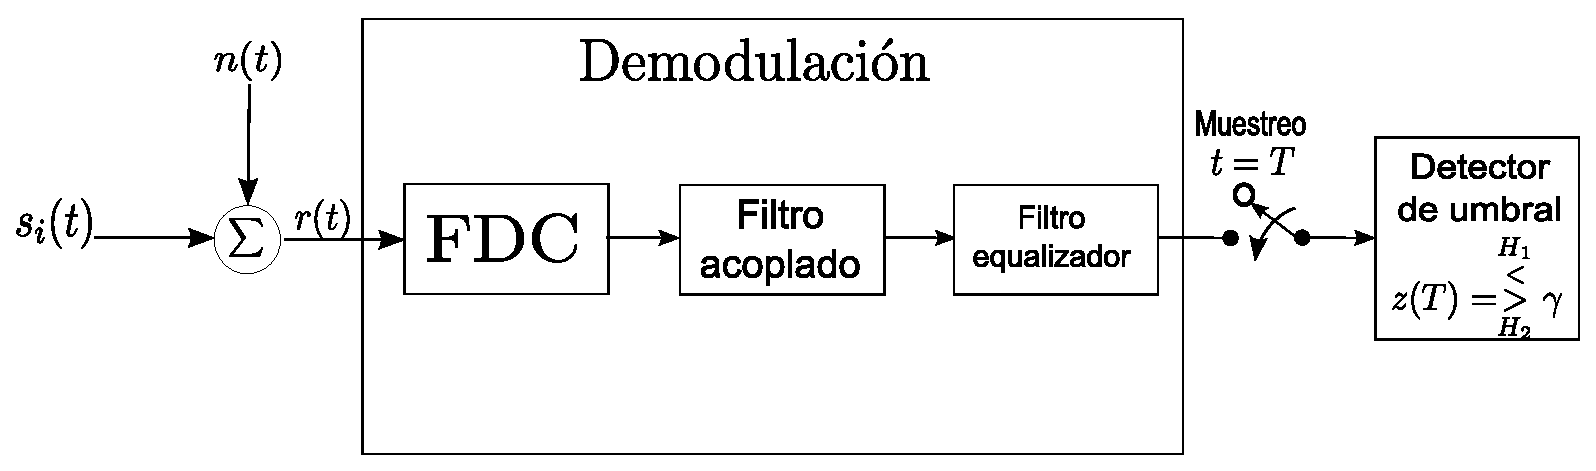
\includegraphics[scale=0.5]{figs/simpledemod}
	\vspace{0.3in}
	\caption{Diagrama simple de un demodulador digital.}
	\label{fig:simpledemod}
\end{figure}

Dentro de la etapa de demodulaci\'on, el bloque de conversi\'on de frecuencia hacia abajo
realiza la operaci\'on de mover la frecuencia central de la se\~nal a otra mas baja. Esta nueva
frecuencia puede ser 0 (DC) o una intermedia. Este bloque normalmente se emplea para se\~nales de
tipo pasa bandas. Su empleo es totalmente opcional ya que se utiliza para acondicionar la frecuencia
de la se\~nal a una que el sistema de detecci\'on pueda utilizar adecuadamente. El siguiente bloque
implementa un filtro acoplado que se utiliza para recuperar los pulsos de banda base con la mejor
taza de se\~nal a ruido (SNR). En algunos casos se utiliza un filtro equalizador para reducir el
fen\'omeno de ISI inducido por el canal y se introduce despu\'es del filtro acoplado. La mayor\'ia de
veces es preferible implementar un solo filtro que realize ambas operaciones para que de esa manera
pueda compensar las distorsiones generadas por ambos, el transmisor y el canal.

Asumiendo que el ruido que contiene la se\~nal es Gauseano, la salida del demodulador en la figura
\ref{fig:simpledemod} entrega la siguiente prueba estad\'istica:

\begin{equation}
z(T)=a_i(T)+n_0(T) \quad i=1,2
\end{equation}

para un sistema binario, donde $a_i(T)$ es la se\~nal deseada, $n_0$ es el ruido y $T$ es la duraci\'on del s\'imbolo. Como
el ruido es un proceso Gauseano aleatorio, $z(T)$ es una variable Gauseana aleatoria que tendr\'a una media de
$a_1$ o $a_2$ dependiendo si un 1 o un 0 binario fue enviado. Con esto podemos expresar las
funciones de densidad de probabilidad condicionales para cada s\'imbolo de la siguiente manera:

\begin{equation}
p(z|s_1)=\frac{1}{\sigma_0
\sqrt{2\pi}}\exp{\left[-\frac{1}{2}\left(\frac{z-a_1}{\sigma_0}\right)^2 \right]}
\end{equation}

y

\begin{equation}
p(z|s_2)=\frac{1}{\sigma_0
\sqrt{2\pi}}\exp{\left[-\frac{1}{2}\left(\frac{z-a_2}{\sigma_0}\right)^2 \right]}
\end{equation}

Una representaci\'on gr\'afica de estas probabilidades condicionales se muestra en la figura
\ref{fig:condpdf}.

\begin{figure}[htp]
\centering
	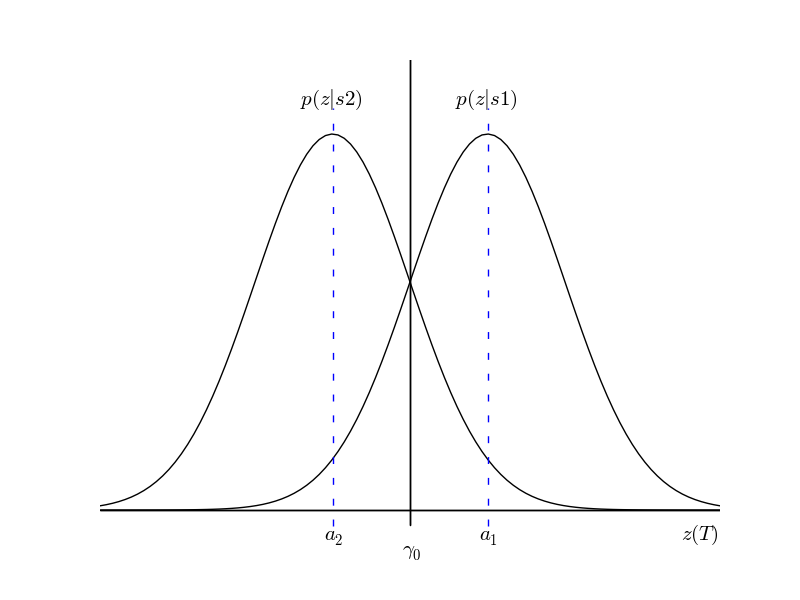
\includegraphics[width=5.5in]{figs/condpdf}
	\caption{Probabilidades condicionales de las funciones $p(z|s_1)$ y $p(z|s_2)$}
	\label{fig:condpdf}
\end{figure}

El eje x representa todo el rango de valores posibles que pueden ser recibidos y las distribuciones
representan la densidad de probabilidad dado que $s_1$ o $s_2$ haya sido transmitido. Debido a que
$z(T)$ es un voltaje proporcional a la energ\'ia del s\'imbolo recibido, entre m\'as grande sea la
magnitud de $z(T)$ habr\'a menos errores en el proceso de decisi\'on de s\'imbolos. Esta decisi\'on
se realiza tomando la hip\'otesis resultante de la medici\'on del umbral dada por la ecuaci\'on
\ref{eq:ineq}\cite{sklar}:

\begin{equation}
z(T)\overset{H_1}{\underset{H_2}{\overset{<}{>}}}\gamma
\end{equation}\label{eq:ineq}

donde $H_1$ y $H_2$ son dos posibles hip\'otesis binarias e indica que la hip\'otesis $H_1$ es la que se
escoge si $z(T)>\gamma$ y $H_2$ se escoge si $z(T)< \gamma$. Esto es equivalente a escoger un 0 o un
1 binario dependiendo si $s_1$ o $s_2$ fue enviado.
%==========================================================================
\section{Modulaci\'on QPSK}

Este m\'etodo de modulaci\'on agrupa la informaci\'on en pares de
bits para ser transmitidos por un canal. Cada par representa lo que se denomina
un s\'imbolo, es decir, un posible estado que puede tomar la se\~nal modulada.
QPSK es derivada de la modulaci\'on PSK que es una de las tres principales
modulaciones digitales:
\begin{itemize}
  \item ASK = \emph{Modulaci\'on por corrimiento de amplitud}
  \item FSK = \emph{Modulaci\'on por corrimiento de frecuencia}
  \item PSK = \emph{Modulaci\'on por corrimiento de fase}
\end{itemize}

La modulaci\'on PSK utiliza una cantidad finita de cambios de fase derivados de
una lista de patrones de bits denominada \emph{alfabeto}. Esta lista se
determina de la siguiente manera:
\begin{equation}\label{eq:levels}
M=2^b
\end{equation}
donde $M$ es el total de elementos en el conjunto y $b$ es la cantidad de bits
asignados a cada elemento del conjunto. El tama\~no del alfabeto lo determina la
aplicaci\'on e implica consideraciones en el espacio entre s\'imbolo en el plano
complejo y la probabilidad de error de bit, y que un alfabeto muy grande aumenta
la probabilidad de errores pero a su vez aumenta la eficiencia espectral de la
transmisi\'on.

La modulaci\'on PSK tiene la siguiente expresi\'on general:
\begin{equation}\label{eq:pskgen}
s(t)=\sqrt{\frac{2E}{T}}\cos(\omega_0t+\phi_i(t))
\end{equation}
donde $E$ es la energ\'ia por s\'imbolo, $T$ es la duraci\'on de cada s\'imbolo,
$\omega_i(t)$ es la frecuencia de la portadora y el t\'ermino $\phi_i(t)$
representa los cambios de fase en la se\~nal. Estos valores son t\'ipicamente
dados por la siguiente expresi\'on:
\begin{equation}\label{eq:levelfase}
\phi_i(t)=\frac{2\pi i}{M}; \qquad i=1,\ldots,M 
\end{equation}
donde $M$ es la cantidad de elementos del alfabeto.

La forma m\'as simple de PSK se llama BPSK. Este esquema utiliza un alfabeto de
dos posibles valores separados por 180 grados. Estos valores se pueden observar
claramente en el diagrama de constelaci\'on mostrado en la figura
\ref{fig:bpskconst}. Este diagrama muestra la se\~nal en forma vectorial,
proyectada en el plano complejo. La parte real se le denomina I, o componente ``en fase'' y
la parte imaginaria se le denomina Q, o componente en ``quadratura''. La se\~nal
BPSK se observa como una se\~nal unidimensional, es decir, \'unicamente tiene
proyecci\'on en el eje X. Cada s\'imbolo puede modular \'unicamente un bit, lo
cual hace esta modulaci\'on ineficiente para aplicaciones que requieran una tasa
de transferencia muy alta.
\begin{figure}[hpt]
\centering
	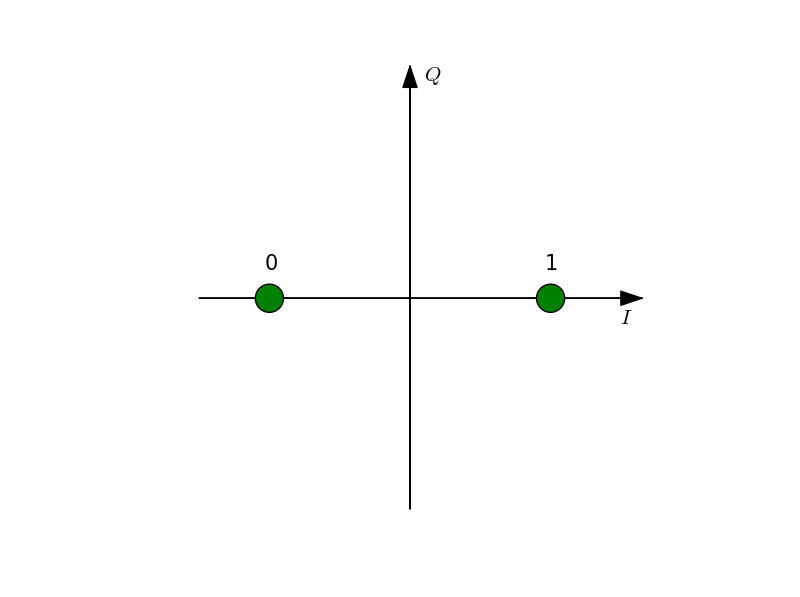
\includegraphics[width=5.5in]{figs/bpsk}
	\caption{Diagrama de constelaci\'on para la modulaci\'on BPSK}
	\label{fig:bpskconst}
\end{figure}

QPSK es otra variaci\'on de PSK que utiliza cuatro puntos en el plano complejo y
por lo tanto, se considera una se\~nal bidimensional ya que tambi\'en tiene
proyecci\'on en el eje Y. Como se mencion\'o anteriormente, este esquema agrupa
los bits en pares por cada s\'imbolo, haciendo esta modulaci\'on espectralmente
m\'as eficiente que BPSK ya que se puede transmitir m\'as informaci\'on
utilizando el mismo ancho de banda. El diagrama de constelaci\'on se muestra en
la figura \ref{fig:qpskconst}.
\begin{figure}[hpt]
\centering
	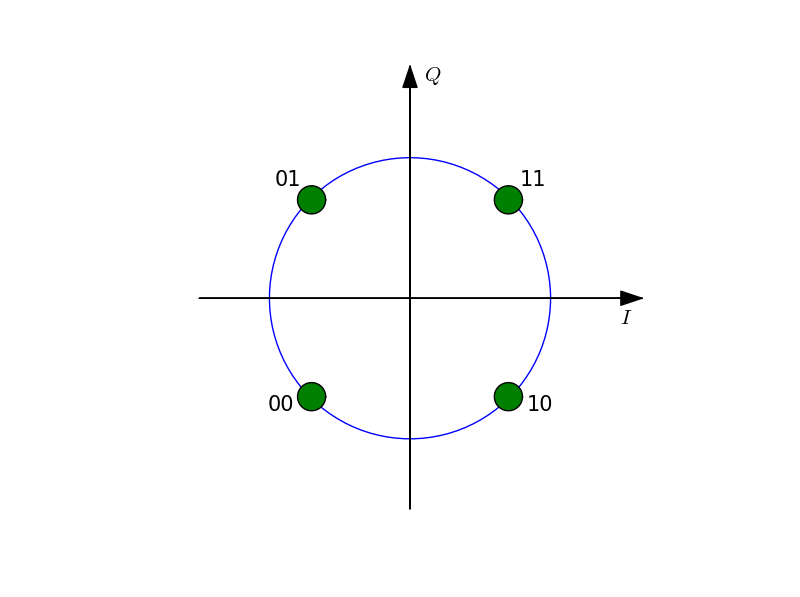
\includegraphics[width=5.5in]{figs/qpsk}
	\caption{Diagrama de constelaci\'on de la modulaci\'on QPSK}
	\label{fig:qpskconst}
\end{figure}

La se\~nal transmitida tiene la siguiente forma \cite{sklar}
\begin{equation}\label{eq:transmit}
s(t)=I(t)\cos(2\pi f_0t)+Q(t)\sin(2\pi f_0t)
\end{equation}
donde $I(t)$ y $Q(t)$ son las se\~nales moduladas y $f_0$ es la frecuencia de la
envolvente.

En el receptor estas dos se\~nales son demoduladas utilizando un demodulador
coherente, es decir, un demodulador que sincroniza la fase de su oscilador
local con la fase de la del oscilador del modulador. Tal receptor multiplica la
se\~nal por separado con una se\~nal seno y coseno para producir los estimados
de $I(t)$ y $Q(t)$ respectivamente.

Matem\'aticamente $I(t)$ puede ser demodulada multiplicando la se\~nal transmitida
con una se\~nal coseno
\begin{equation}
\begin{aligned}
r_i(t)&=s(t)\cos(2\pi f_0t)\\
&=I(t)\cos(2\pi f_0t)\cos(2\pi f_0t)+Q(t)\sin(2\pi f_0t)\cos(2\pi f_0t)
\end{aligned}
\end{equation}
Utilizando las identidades trigonom\'etricas
\begin{equation}
\begin{aligned}
\cos\theta\cos\varphi&=\frac{1}{2}[\cos(\theta+\varphi)+\cos(\theta-\varphi)]\\
\sin\theta\cos\varphi&=\frac{1}{2}[\sin(\theta+\varphi)+\sin(\theta-\varphi)]
\end{aligned}
\end{equation}
se puede escribir
\begin{equation}
\begin{aligned}
r_i(t)&=\frac{1}{2}I(t)[1+\cos(4\omega_0t)]+\frac{1}{2}Q(t)\sin(4\omega_0t)\\
r_i(t)&=\frac{1}{2}I(t)+\frac{1}{2}[I(t)\cos(4\omega_0t)+Q(t)\sin(4\omega_0t)]
\end{aligned}
\end{equation}

Aplicando un filtro pasa bajas a $r_i(t)$ se pueden eliminar los t\'erminos de
frecuencia (los que tienen el t\'ermino $\omega_0$)dejando \'unicamente el
t\'ermino $I(t)$. Similarmente se puede multiplicar $s(t)$ por una se\~nal
senoidal y luego por un filtro pasa bajas para obtener $Q(t)$.

%==========================================================================
\section{Tasa de error de bits QPSK}
El estudio de la tasa de error de bits es de gran importancia ya que nos proporciona una medida del
rendimiento del sistema de comunicaciones. Esta medida se interpreta en t\'erminos de probabilidad de
error del s\'imbolo enviado $P_E$ dado que fue corrompido por el ruido del canal. El ruido se puede
definir como un disturbio no deseable en la se\~nal que se est\'a transmitiendo. Este fen\'omeno
siempre existe en un canal de transmisi\'on y generalmente no se puede evitar, por lo que es
necesario tomarlo en cuenta durante el dise\~no de un sistema de comunicaci\'on.


%==========================================================================

\section{Herramientas de medici\'on de desempe\~no}
Las herramientas que se mencionan en \'esta secci\'on proporcionan un panorama completo del
rendimiento de un sistema de comunicaciones, ya sea de la etapa de transmisi\'on o recepci\'on y
son ampliamente utilizadas para verificar el an\'alisis te\'orico o pr\'actico.

\subsection{Diagrama de ojo}
Una manera eficiente de visualizar la calidad de la se\~nal en el receptor es por medio del diagrama
de ojo. Este diagrama contiene todas las posibles secuencias de bits que muestran debilidades en el
dise\~no del sistema. Un ejemplo se muestra en la figura \ref{fig:eyeform}\cite{foster}.

\begin{figure}[htp]
\centering
	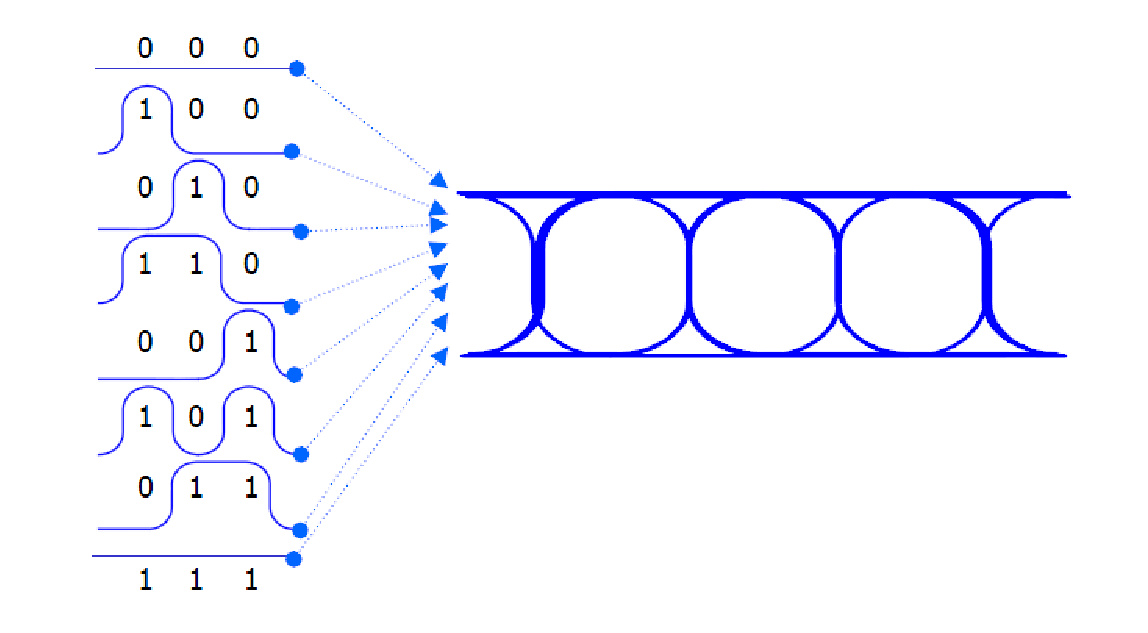
\includegraphics[width=5.5in]{figs/eyeform}
	\caption{El diagrama de ojo formado al sobreponer varias secuencias de bits}
	\label{fig:eyeform}
\end{figure}

La forma convencional de generar el diagrama de ojo es por medio de un osciloscopio en modo de
persistencia. Cada captura es obtenida mediante un reloj de sincronizaci\'on obtenida de la misma
forma de onda recibida. El modo de persistencia causar\'a que los trazos de la onda se sobrepongan
una con la otra hasta formar el patr\'on de ojo sobre la pantalla. Los par\'ametros que se pueden
medir se muestran en la figura \ref{fig:eyeparams}\cite{breed}.

La distorsi\'on en el tiempo de muestreo es generada por el fen\'omeno de ISI. La diferencia en
tiempo pico a pico de los cruces por cero se le conoce tambi\'en como \emph{jitter}. El momento
\'optimo para iniciar el muestreo de un s\'imbolo es en la parte que est\'a m\'as abierta del ojo. Conforme el
SNR es m\'as bajo el ojo comenzar\'a a cerrarse haciendo as\'i m\'as dif\'icil y, por concecuencia,
m\'as err\'oneo el muestreo de la se\~nal recibida.

\begin{figure}[hbp]
\centering
	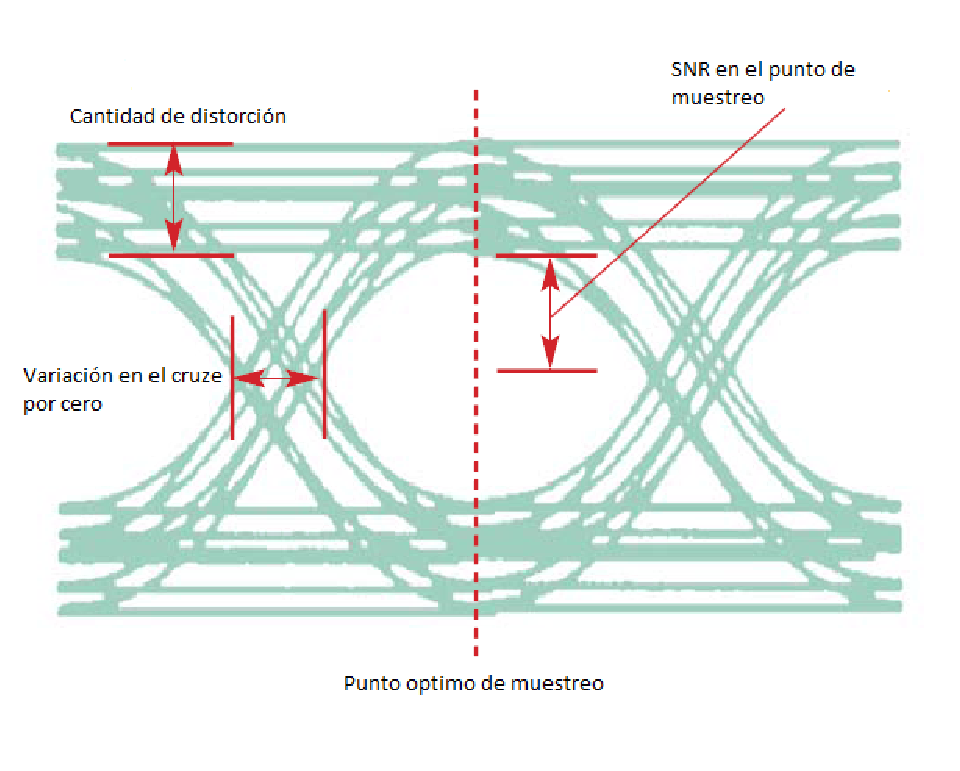
\includegraphics[width=4in]{figs/eyeparams}
	\caption{Par\'ametros de medici\'on del diagrama de ojo.}
	\label{fig:eyeparams}
\end{figure}

\subsection{Espectrograma}
El espectrograma, tambi\'en conocido como gr\'afica de cascada (\emph{waterfall}), muestra las variaciones de la densidad
espectral de la se\~nal a trav\'es del tiempo. Utiliza tres par\'ametros para mostrar una imagen representando la distribuci\'on
espectral: el tiempo, la frecuencia y la amplitud. El eje X representa el tiempo, el eje Y la frecuencia y una escala de colores
muestra la intensidad de cada punto en la imagen. Los ejes X y Y pueden ser invertidos para visualizar la imagen de abajo hacia
arriba. Un ejemplo de un espectrograma se muestra en la figura \ref{fig:spectrogram}.

\begin{figure}[tp]
\centering
	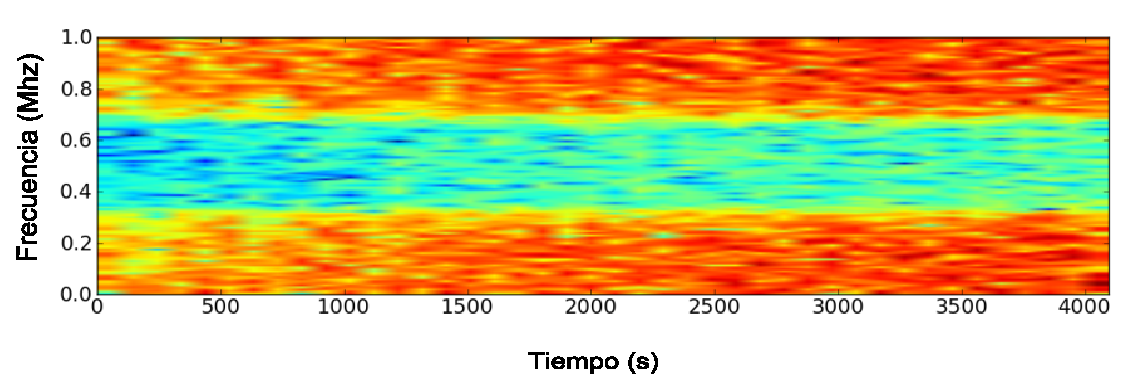
\includegraphics[width=5.5in]{figs/spectrogram}
	\vspace{0.3in}
	\caption{Ejemplo de un espectrograma.}
	\label{fig:spectrogram}
\end{figure}

%==========================================================================
\section{Concepto de radio reconfigurable por software}

El concepto del radio definido por software fue primeramente establecido por Joseph Mitola\citeyear{mitola}. Normalmente se les
llaman SDR por sus siglas en ingles (\emph{Software Defined Radio}). Este tipo de radio consiste en reemplazar los moduladores,
filtros, amplificadores, etc., de un sistema de RF t\'ipico y reemplazarlos por software. La idea principal es conectar la antena
lo m\'as cerca al procesador. Un sistema b\'asico podr\'ia consistir en una PC, una tarjeta de sonido y alguna circuiter\'ia de RF
para acoplar la antena. Un diagrama a bloques del sistema b\'asico de un SDR se muestra en la figura \ref{fig:sdr}. Para un
sistema receptor SDR lo \'unico que se tiene que cambiar es el bloque de DAC por un ADC. Gracias al procesamiento digital de
se\~nales dentro del procesador, este tipo de radio puede trabajar con diferentes tipos de se\~nales, codificaciones y
modulaciones con tan solo cambiar el software. Algunas ventajas que estos sistemas ofrecen son: bajo costo, un factor de tama\~no
m\'as peque\~no y una mayor facilidad de mantenimiento y actualizaci\'on.

\begin{figure}[tp]
\centering
	\begin{tikzpicture}
		\node (cpu) [sc] {Procesador General};
		\node (dac) [sc, right=of cpu] {DAC}
			edge [<-, very thick] (cpu);
		\node (ant) [sc, right=of dac] {Antena}
			edge [<-, very thick] (dac);
	\end{tikzpicture}
	\vspace{0.3in}
	\caption{Diagrama a bloques de un sistema ideal de SDR}
	\label{fig:sdr}
\end{figure}

Los requerimientos del procesador general para la implementaci\'on de algoritmos que llevan a cabo las tareas de modulaci\'on,
codificaci\'on, etc., son tan grandes que hoy en d\'ia aun no hay plataformas suficientemente poderosas para implementar el SDR
ideal. Sin embargo, los avances tecnol\'ogicos de hoy est\'an permitiendo el desarrollo de nuevos procesadores con capacidades
suficientemente poderosas para esta aplicaci\'on en especial. Algunos procesadores como el OMAP3 de la Texas Instruments
\cite{ti} y los FPGAs Virtex de Xilinx \cite{lyrtech} ofrecen plataformas altamente flexibles y con capacidad suficiente para la
implementaci\'on de algoritmos sofisticados de modulaci\'on y codificaci\'on, as\'i como tambi\'en filtrado entre otros.

Algunas de las \'areas donde se aplican los conceptos de los SDRs son por
ejemplo en el \'area militar. El sistema de comunicaciones del ej\'ercito
militar de Estados Unidos est\'a siendo remplazado por un sistema basado en SDRs
con la capacidad de poder establecer un enlace sin importar el tipo de radio y
con capacidad de trabajar con diversas redes de comunicaci\'on. La ventaja
principal que los l\'ideres militares ven en el uso de SDRs es la habilidad de
poder configurar el sistema para utilizar diversas capas de protocolos y
formatos sin actualizar el hardware. El programa JTRS (por sus siglas en ingles
\emph{Joint Tactical Radio Systems}) es un SDR que permitir\'a a los soldados
poder comunicarse con una amplia cantidad de redes de comunicaci\'on as\'i como
redes que utilizan arquitecturas viejas \cite{mchale}. El plan de
este programa es remplazar el hardware tradicional de los radios utilizados en
el ej\'ercito militar con dispositivos que puedan emular las capacidades de
cualquier radio.

\begin{figure}[pt]
\centering
	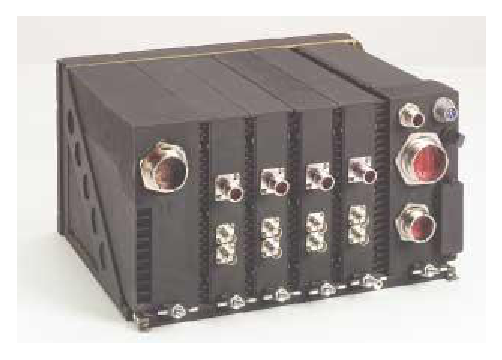
\includegraphics[scale=0.7]{figs/jtrs}
	\caption{Hardware proporcionado por Rockwell Collins para el cluster JTRS
	(Mchale, 2004)}
	\label{fig:jtrs}
\end{figure}

En la figura \ref{fig:jtrs} se muestra el hardware proporcionado al ej\'ercito
militar por el sector de comunicaciones de Rockwell Collins.

Otro ejemplo de una aplicaci\'on en el \'area acad\'emica es el proyecto Hydra
de la Universidad de Texas en Austin \cite{hydra}. Este proyecto consiste en un
sistema de pruebas enfocado a redes que soportan m\'ultiples saltos
inal\'ambricos y donde la red toma ventaja de t\'ecnicas sofisticadas como OFDM
y MIMO. El sistema se basa en el proyecto de \emph{GNURadio} y su plataforma de
desarrollo USRP \cite{ettus} para la implementaci\'on de la etapa de RF y del
software. La estructura de este sistema se muestra en la figura \ref{fig:hydra}.

\begin{figure}[hpt]
\centering
	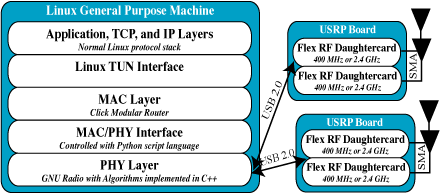
\includegraphics[scale=0.7]{figs/hydra}
	\vspace{0.5in}
	\caption{Diagrama a bloques de un nodo del sistema Hydra (Wireless
	Comm Group, 2007)}
	\label{fig:hydra}
\end{figure}
